\documentclass{article}

\usepackage[italian]{babel}
\usepackage[T1]{fontenc}
\usepackage[utf8]{inputenc}
\usepackage{hyperref}
\hypersetup{
	colorlinks=true,
	linkcolor=blue
	}
\usepackage{graphicx}

\title{{\huge Visualizzatore di aule libere}}
\author{Arianna Masciolini, matricola 285025\\ Tommaso Ricci, matricola XXXXXX}
\date{A.A. 2016-2017}


\begin{document}
	\maketitle
	\newpage
	\tableofcontents
	\newpage
	\part{Introduzione al progetto}
	\section{Abstract}
	Rivolta principalmente agli studenti che utilizzano le aule per la didattica frontale anche per lo studio di gruppo, l'applicazione permette di individuare le aule libere del Dipartimento di Matematica ed Informatica dell'Università degli Studi di Perugia grazie ad una semplice interfaccia grafica in cui le informazioni sono visualizzate sulle planimetrie dell'edificio.
	\section{Obiettivi}
	Obiettivo principale del progetto è, pertanto, fornire agli utenti un'alternativa rapida ed efficace alla consultazione del tabellone orario. Lo studente avrà in tasca le informazioni essenziali, da consultare agevolmente anche in mobilità quando gli fosse utile conoscere in anticipo la situazione.
	\paragraph{Prospettive e sviluppi futuri}
	Nelle versioni successive, ci si propone di aggiungere svariate funzionalità all'applicativo; innanzitutto la possibilità, per gli utenti, di comunicare informazioni sullo stato delle aule in tempo reale, in modo da rendere più accurati e completi i dati visualizzati. In tale scenario, ci si propone inoltre di tracciare, con lo stesso sistema, lo stato di occupazione dei tavoli collocati nei vari pianerottoli. Obiettivo a lungo termine, infine, è quello di creare una procedura per la creazione di mappe, così da facilitare la diffusione di questo sistema in contesti esterni a quello del DMI.
	\newpage
	\part{Documento di analisi}
	\section{Analisi dei requisiti e descrizione delle soluzioni adottate} 
	La decisione di realizzare un applicativo Android si deve alla sua grande diffusione nel mondo dei dispositivi mobili, ai quali il progetto è destinato.
	Occorre innanzitutto che l'applicazione, dalle funzionalità volutamente minimali, recuperi i dati relativi alla gestione delle aule dipartimentali dalle fonti ufficiali. Una prima possibilità per ottenere quanto descritto è il web scraping: i dati sono infatti pubblicati in una pagina del sito web del Dipartimento, che offre ai visitatori un servizio in parte analogo a quello che l'applicazione si propone di adattare alle esigenze degli studenti, rivolto però principalmente agli insegnanti, che autenticandosi possono prenotare le aule. A questa strategia si è preferita però l'interrogazione diretta del database mySQL che contiene in forma più completa e maneggevole le informazioni relative alle prenotazioni delle aule dipartimentali: il database \textbf{mrbs}. $Segue$
	Per quel che riguarda l'interfaccia utente, sono di massima importanza leggibilità e facilità d'uso. Si è scelto pertanto di utilizzare, ripulite da ogni dettaglio superfluo, le planimetrie del DMI, utilizzando un color coding intuitivo per descrivere, tramite immagini in sovraimpressione, lo stato delle diverse classi. Viste le dimensioni limitate degli schermi degli smartphone, ogni schermata mostra un solo piano dell'edificio. Infine, grazie ad un sistema mappatura delle planimetrie, al tocco della superficie di un'aula l'utente potrà visualizzare alcune informazioni aggiuntive riguardo il suo utilizzo o, nel caso di laboratori e biblioteche, gli orari di apertura e chiusura.
	\paragraph{Metodologie di sviluppo}
	La metodologia adottata per lo sviluppo dell'app Android si basa sull'approccio incrementale, più efficiente e gratificante rispetto al tradizionale modello a cascata, specialmente per sviluppatori alle prime armi. Per ragioni analoghe, si è deciso di coniugare i rilasci successivi con l'idea di pair programming.
	Al fine di semplificare la collaborazione tra i due autori del progetto quando non si è rivelato possibile lavorare alla stessa postazione e per facilitare, in futuro, la diffusione e il miglioramento dell'applicazione, si è deciso di pubblicarne il codice sorgente, disponibile all'indirizzo \url{https://github.com/Disorganizzazione/AuleLibere}.
	\section{Requisiti di sistema}
	\paragraph{Minimi}
	\paragraph{Consigliati}
	\newpage
	\part{Documentazione UML}
	\section{Diagramma di classe}
	\newpage
	\section{Casi d'uso}
	Nel diagramma dei casi d'uso si sono volute lasciare, per completezza, anche indicazioni sulle azioni che l'utente potrà compiere nelle versioni future dell'applicazione.\\
	\begin{figure}[h]
		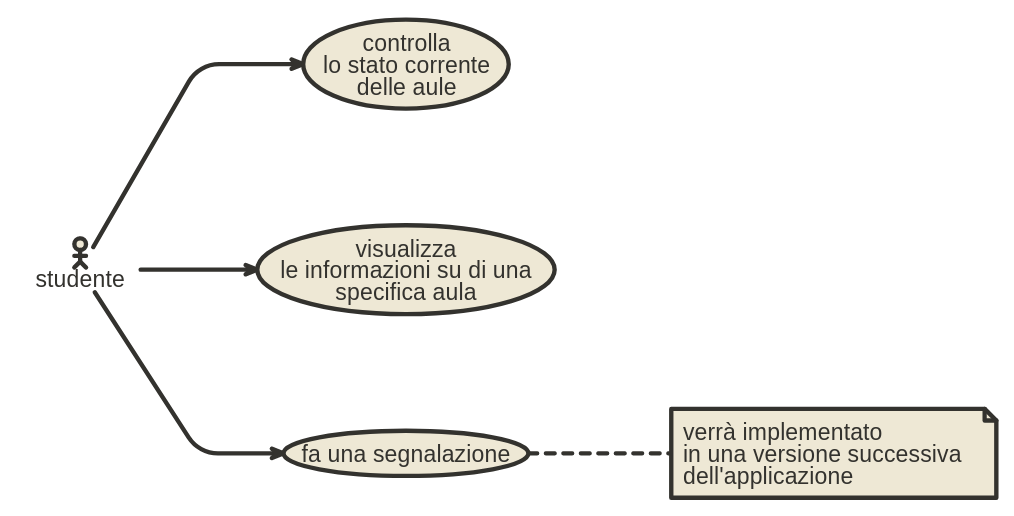
\includegraphics[scale=0.40]{casiduso}
		\centering
		\caption{Diagramma dei casi d'uso}
	\end{figure}
	\newpage
	\section{Diagramma di sequenza}
	\newpage
	\section{Diagramma di collaborazione}
	\newpage
	\section{Diagramma di stato}
	Lo stato di un'aula varia in modo ciclico: solo per rispettare le convenzioni, si è comunque scelto come stato iniziale quello in cui l'aula è chiusa; tuttavia la scelta è del tutto arbitraria, per cui si è rinunciato a definire anche uno stato finale distinto, dal momento che tale decisione avrebbe costituito una forzatura.\\
	\begin{figure}[h]
		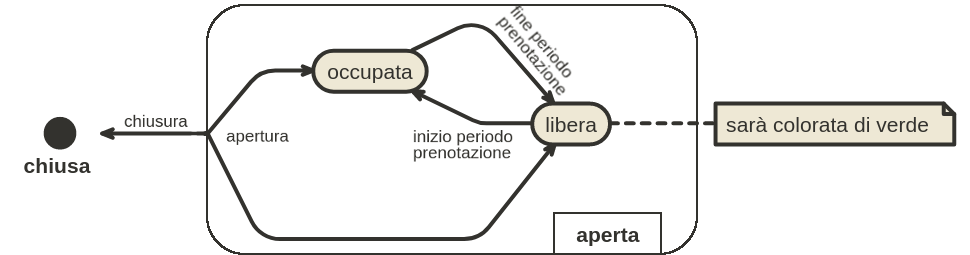
\includegraphics[scale=0.45]{stato}
		\centering
		\caption{Diagramma di stato relativo ad un'aula}
	\end{figure}
	\newpage
	\section{Diagramma di attività}
	\newpage
	\part{Test funzionali}
	\newpage
	\part{Design pattern}
	\newpage
	\appendix
	\part{Glossario}
\end{document}
